% !TEX program = xelatex

\documentclass[12pt,a4paper]{article}

\usepackage{amsthm,amsfonts,amssymb,bm}
\usepackage[fleqn]{amsmath}
\addtolength{\textheight}{2.0cm}
\addtolength{\voffset}{-2cm}
\addtolength{\hoffset}{-1.5cm}
\addtolength{\textwidth}{4.0cm}

%\allowdisplaybreaks

\usepackage{subeqnarray}
\usepackage{mathrsfs}
%\usepackage{color}
%\usepackage{url}
%\usepackage{ulem}
\usepackage{indentfirst}
%\usepackage{textcomp}
%\usepackage{graphics}
\usepackage{graphicx}
\usepackage[hang,small,bf]{caption}
\setlength{\captionmargin}{50pt}
%\usepackage{pdfpages}
\usepackage{enumerate}

\usepackage{morefloats} % This package is to reslove the too many unprocessed floats error.



%%Here is the configuration for chinese. 
%\usepackage[cm-default]{fontspec}
%\usepackage{xunicode}
%\usepackage{xltxtra}
%\setmainfont{AR PL UKai CN}
%\setsansfont[BoldFont=SimHei]{KaiTi_GB2312}
%\setmonofont{NSimSun}

%\XeTeXlinebreaklocale "zh"
%\XeTeXlinebreakskip = 0pt plus 1pt


%\usepackage{tikz}
%\usetikzlibrary{mindmap,trees}


\graphicspath{{figures/}{files/}}

\begin{document}
\title{Summary}
\author{MA Lei}
\maketitle


\newcommand{\dd}{\mathrm d}
\newcommand{\HH}{\mathcal H}
\newcommand{\CN}{{\it Cosmologia Notebook}}
\newenvironment{eqnset}
{\begin{equation}\left \bracevert \begin{array}{l}}
{\end{array} \right. \end{equation}}

\newenvironment{eqn}
{\begin{equation}\left \bracevert \begin{array}{l}}
{\end{array} \right. \end{equation}}





\section{Objectives}

For LCDM, interacting models, and CPL, calculate

\begin{itemize}
\item
$\xi$ range for varying EoS while fixing $\Omega m0$
\item
$\xi$ range for varying $\Omega m0$ or r, while fixing $\omega$
\item
Does $\xi>0$ means energy transfer to dark energy in this method?
\end{itemize}



\section{Background}


Deceleration parameter reads
\begin{equation}
q(z) = -1 + \frac{1+z}{H}\frac{\mathrm dH}{\mathrm dz}
\end{equation}


% subsection sube (end)
For interaction models, the Friedmann equaitons,
\begin{subeqnarray}
\dot \rho_c +3 H \rho_c &=& Q_c\\
\dot \rho_d + 3 H (1+w)\rho_d &=& -Q_c\label{eqn-rhoc_fund}
\end{subeqnarray}





\paragraph{$Q_c = \xi H \rho_c$} Background equations,
\begin{subeqnarray} \Omega m&=& \Omega m0 (1+z)^{3-\xi} \\
\Omega d = (\Omega d0 + \frac{\xi}{3w + \xi} \Omega m0 )(1+z)^{3(1+w)} + \frac{-\xi}{\xi + 3w}\Omega m &=& \bar{\Omega d0} (1+z)^3 + \frac{-\xi}{\xi + 3w}\Omega m \label{eqn-rhom}
\end{subeqnarray}

\paragraph{$Q_c=\xi H \rho_d$}  
\begin{subeqnarray}
\Omega m = (\Omega m0 + \frac{\xi}{\xi + 3w} \Omega d0)(1+z)^3 + \frac{-\xi}{\xi + 3w}\Omega d &=& \bar{\omega m0}(1+z)^3 +\frac{-\xi}{\xi + 3w}\Omega d \\
\Omega d &=& \Omega d0 (1 + z)^{3(1+w)+\xi}\label{eqn-rhod}
\end{subeqnarray}

Eqn \ref{eqn-rhom} and eqn \ref{eqn-rhod} shows that the coupling constant has two effects,
\begin{enumerate}
\item
Change the amplitude of the evolution of matter or dark energy energy density.
\item
Transfer energy between DE and DM.
\end{enumerate}

\subsection{Some definitions}
\begin{enumerate}
\item
For short
\[r=\frac{\Omega m0}{\Omega d0}\]
\end{enumerate}

\paragraph{CPL}
EoS is 
\[ w=w0+w1\frac{z}{1+z} \]



\paragraph{Classification}

\begin{figure}[htpb]
\centering
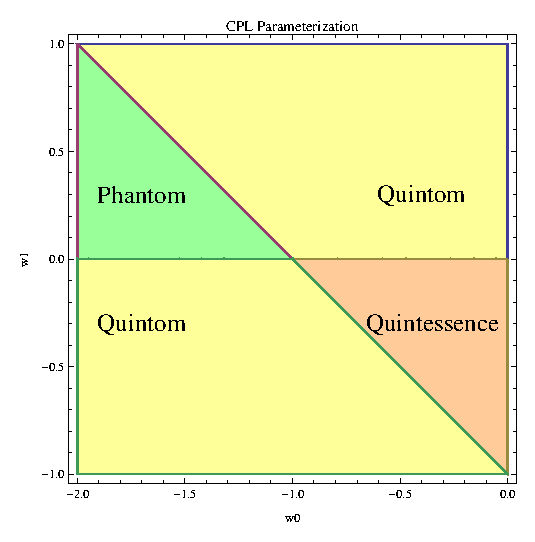
\includegraphics[width=400pt]{CPL_Classification.eps}
\caption{CPL classification}\label{fig-CPL_Classification}
\end{figure}

Figure \ref{fig-CPL_Classification} shows how to category the dark energy models in CPL parametrization.


\section{Data \& Method}

\subsection{Data}

\paragraph{LCDM Parameters}
From WMAP, $\Omega m0 = 0.265$

\paragraph{Constraints}
$\Omega m0=0.247 (+0.013,-0.013)$; Transition redshift 0.426 (+0.082, -0.050).(arXiv:1205.4688, arXiv:astro-ph/0611572).

In ($\Omega m0$, Transition redshift) plane, allowed region is a rectangle centred at (0.274, 0.426) with two diagonal points (0.261, 0.376) and (0.287, 0.508).


\paragraph{CPL}
$\Omega m0=0.269 (+0.017, -0.008)$, $w0 = -0.97 (+0.12, -0.07)$, $w1=0.03 (+0.26, -0.75)$



\section{Results}

Check the files in files folder.

\subsection{$Q_c=\xi H \rho_c$}


Results table

\begin{figure}[htpb]
\centering
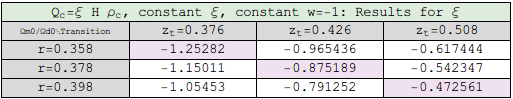
\includegraphics[width=500pt]{rhoc_ICC_table1.png}
\caption{ICC Result table}
\end{figure}


\begin{figure}[htpb]
\centering
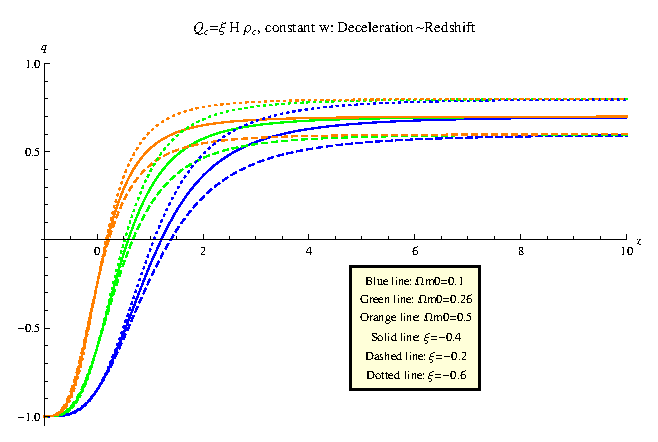
\includegraphics[width=500pt]{rhoc_DecelerationPara.eps}
\caption{Deceleration parameter}\label{fig-rhoc_DecPara}
\end{figure}


Figure \ref{fig-rhoc_DecPara} shows that 
\begin{enumerate}[\bf\tiny{$\rho_c$-Dec}-1]
\item  
The universe decelerates faster at the early stage for smaller interaction constant $\xi$ even they have the same matter fraction.
\item
For the same $\xi$, the deceleration converge ($q=(1-\xi)/2$ with $3w+\xi < 0$) at early time.
\end{enumerate}



\begin{figure}[htpb]
\begin{center}$
\begin{array}{cc}
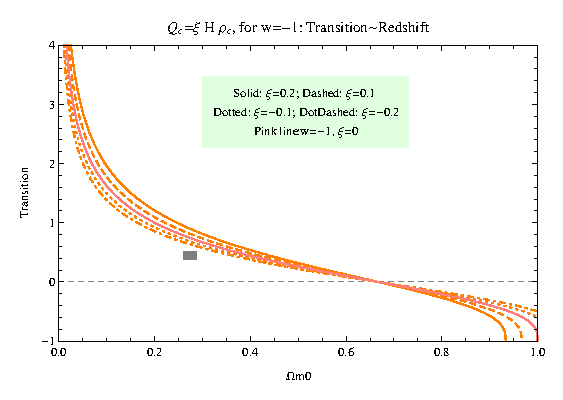
\includegraphics[width=250pt]{rhoc_TransVSOmegam1.eps} &
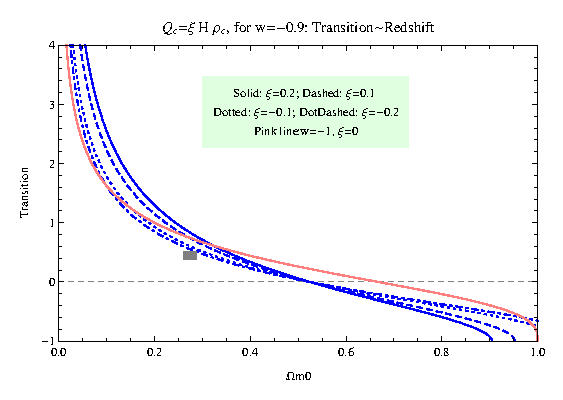
\includegraphics[width=250pt]{rhoc_TransVSOmegam2.eps}
\end{array}$
\end{center}
\caption{Transition redshift.}\label{fig-rhoc_TransVSOmegam}
\end{figure}



Figure \ref{fig-rhoc_TransVSOmegam} shows

\begin{enumerate}[\bf\tiny{$\rho_c$-Trans}-1]
\item
Transition happens earlier when matter fraction is smaller. Matter is against DE's pressure.
\item
Transition is later when $\xi$ is smaller.Energy transfers to DE when $\xi$ is negative, then why later transition? \footnote{Reasons below.
All solutions of equation \ref{eqn-rhoc_fund} have the same value at $z=0$, i.e. now. Equation \ref{eqn-rhoc_fund}a tells us a positive $\xi$ leads to smaller energy density of dark matter at early time of the universe, thus dark energy takes over quickly if the transition happens before today.
(For more details, calculation are shown in supplement\_ 08-10.pdf file.)
}
\end{enumerate}




\begin{figure}[htpb]
\centering
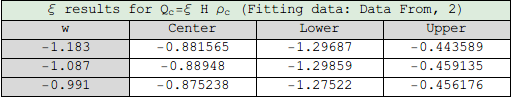
\includegraphics[width=500pt]{rhoc_ICC_table3.png}
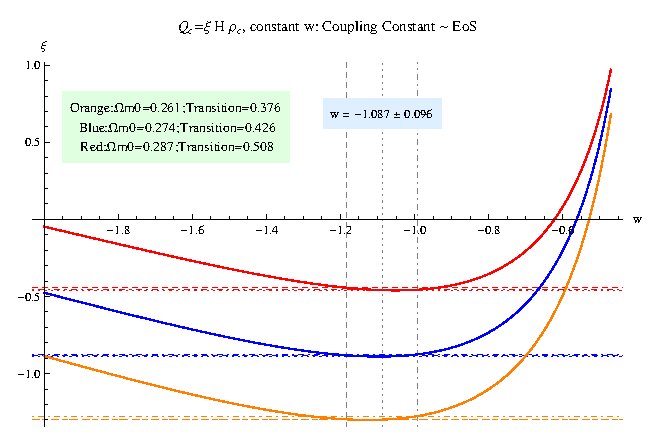
\includegraphics[width=500pt]{rhoc_ICC_xiVSw.eps}
\caption{Interacting coefficient for $Q_c=\xi H\rho_c$}\label{fig-rhoc_ICC_xiVSw}
\end{figure}

\begin{figure}[htpb]
\centering
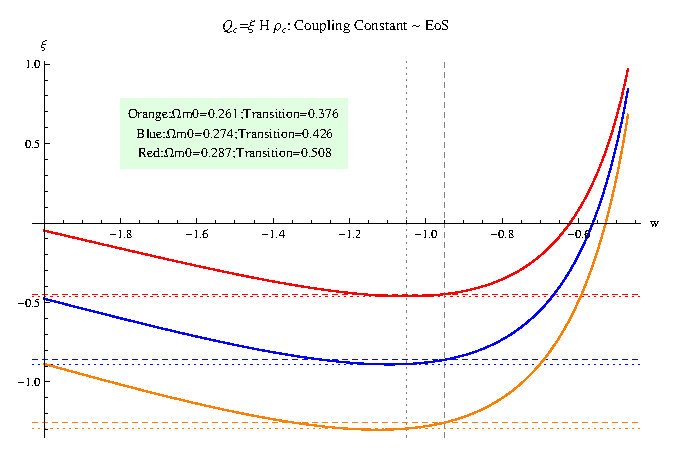
\includegraphics[width=500pt]{rhoc_ICC_xiVSw2.eps}
\caption{Interacting coefficient for $Q_c=\xi H\rho_c$}\label{fig-rhoc_ICC_xiVSw2}
\end{figure}


Figure \ref{fig-rhoc_ICC_xiVSw} and figure \ref{fig-rhoc_ICC_xiVSw2} (vertical lines are $w=-1\pm 0.05$) show the value of $\xi$ for different EoS. 

Results from this figure:

(EoS is -1 within 5%: (-1.05,-0.95)): 
w=-1  (-1.279,-0.457) center:-0.878 ;
w=-1.05  (-1.293,-0.461) center:-0.887 ;
w=-0.95  (-1.255,-0.447) center:-0.860 ;

\begin{enumerate}[\bf\tiny{$\rho_c$-xiVSw}-1]
\item
NOT monotonic. The result of $\xi$ is greatly affected by $\Omega m0$. In correspondence with another 
\item
For different $\Omega m 0$, $\xi$ values deviate greatly form each other at small $w$.
\end{enumerate}




\begin{figure}[htpb]
\centering
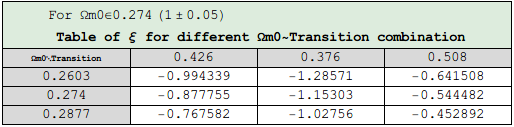
\includegraphics[width=450pt]{rhoc_ICC_table4.png}
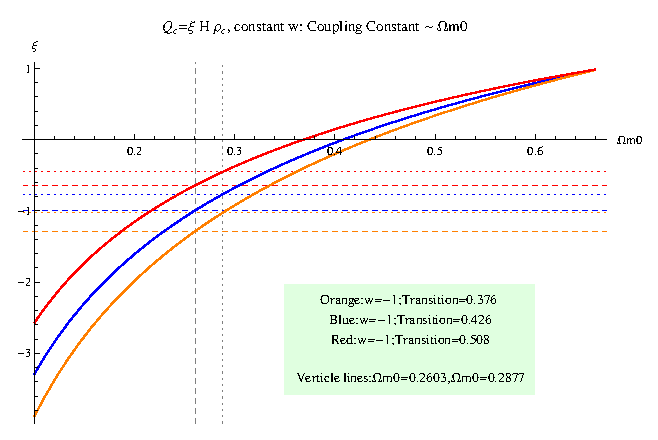
\includegraphics[width=350pt]{rhoc_ICC_xiVSOmegam0.eps}
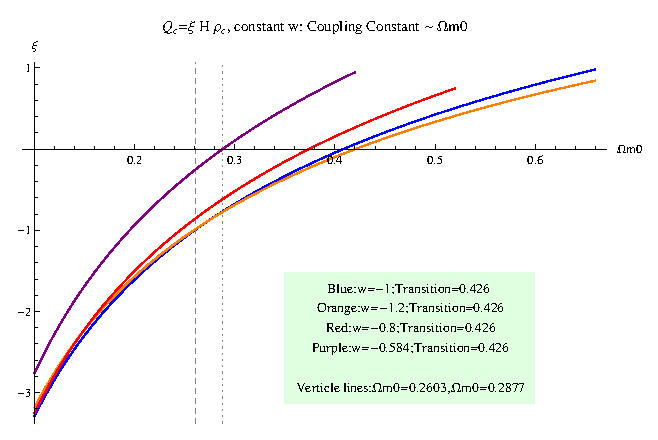
\includegraphics[width=350pt]{rhoc_ICC_xiVSOmegam02.eps}
\caption{Interacting coefficient changing with $\Omega m0$ for $Q_c=\xi H\rho_c$}\label{fig-rhoc_ICC_xiVSOmegam0}
\end{figure}

Figures \ref{fig-rhoc_ICC_xiVSOmegam0} show how do we constrain $\xi$ and how do EoS change our constrain results with the transition fixed.
\begin{enumerate}[\bf\tiny{$\rho_c$-xiVS$\Omega m0$}-1]
\item
The smaller, the more difference among $\xi$ values of different EoS. Reason for this is less matter has less effect on the evolution thus the property of dark energy determines more about the transition.
\item
Second figure shows
\begin{enumerate}
\item [+]
System with smaller $w$ needs smaller coupling to achieve the same transition time, as expected.
\item[+]
So we give the result that $w \in (-0.58406, -0.3334)$ if we constrain $\Omega m0 = 0.2603$ and transition redshift 0.426.
\end{enumerate}
\end{enumerate}

\subsection{$Q_c=\xi H\rho_c$, CPL}


For a flat universe, choose the parameters {w0=-1.02,w1=0.6}, the region for interation cosntant $\xi$ should be  (-1.04,-0.21) with a center at -0.64, derived from the (transition redshift, $\Omega m0$) plane, while a result of (-1.01, -0.23) with a center at -0.63, derived from (transition redshift, $\Omega m0$/%\Omega d0%) plane.


First let's have a look at the deceleration parameter.

\begin{figure}[htpb]
\centering
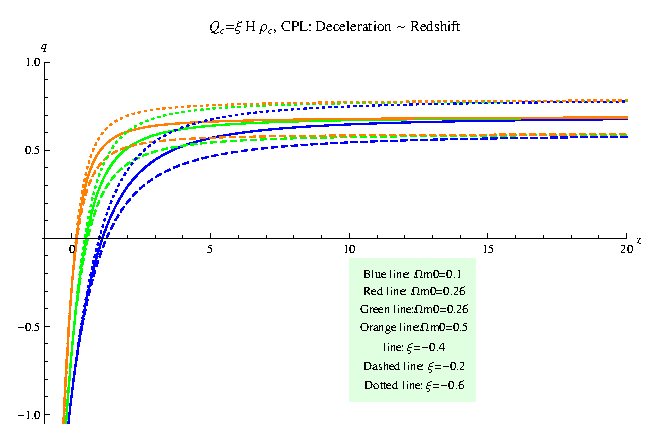
\includegraphics[width=500pt]{rhoc_ICCPL_DecPara.eps}
\caption{Deceleration parameters for ICCPL ($Q_c=\xi H \rho_c$ with CPL parametrized EoS)}\label{fig-rhoc_ICCPL_DecPara}
\end{figure}

Figure \ref{fig-rhoc_ICCPL_DecPara} is right similar to constant EoS situation.


\begin{figure}
\centering
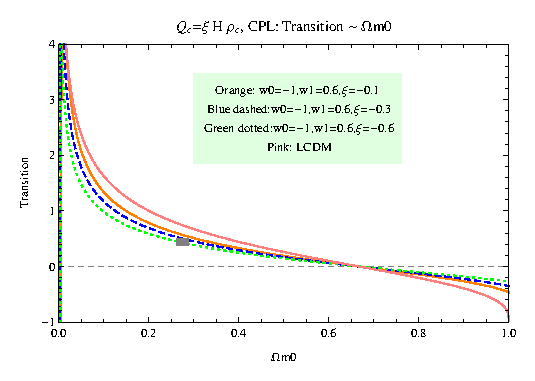
\includegraphics[width=250pt]{rhoc_ICCPL_TransVSOmegam01.eps}
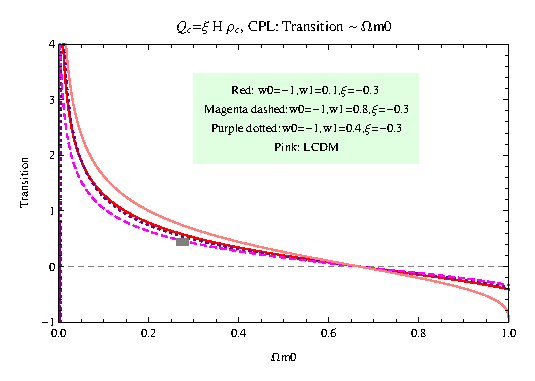
\includegraphics[width=250pt]{rhoc_ICCPL_TransVSOmegam02.eps}
\caption{The effect of EoS parameters on Transition and $\Omega m0$}\label{fig-rhoc_ICCPL_TransVSOmegam0}
\end{figure}

Figures \ref{fig-rhoc_ICCPL_TransVSOmegam0} show 
\begin{enumerate}[\bf\tiny{$\rho_c$-ICCPL-TVS$\Omega m0$}-1]
\item
Coupling acts on these model similar to constant EoS model.
\item
The change in $w1$ has a similar effect with the change of $\xi$. Larger $w1$ corresponds to smaller $\xi$. The reason for this is both negative $\xi$ and larger $w1$ enhances the energy density of dark energy (check using the CPL EoS).
\end{enumerate}



\begin{figure}[!htpb]
\centering
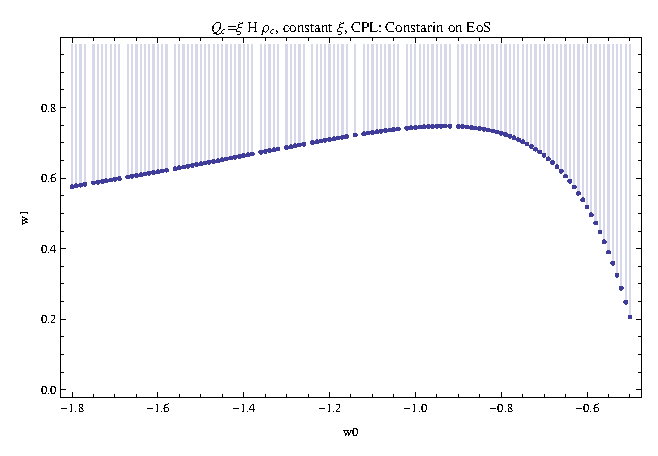
\includegraphics[width=500pt]{ICCPL_w1VSw0_LowerBound.eps}
\caption{Lower bound in the W1~w0 parameter space}\label{ICCPL_w1VSw0_LowerBound}
\end{figure}

The dots in figure \ref{ICCPL_w1VSw0_LowerBound} are the data set of $\xi=0$. If we need $\xi<0$, i.e., energy transfers from dark matter to dark energy, the allowed parameter space is the striped area.




\subsubsection{Quintom}

(Figures \ref{fig-rhoc_ICCPL_Quintom_EoS}, \ref{fig-rhoc_ICCPL_Quintom_TransVSOmegam0}, \ref{fig-rhoc_ICCPL_Quintom_xiVSOmegam0}, \ref{fig-rhoc_ICCPL_Quintom_TransVSOmegam02}, \ref{fig-rhoc_ICCPL_Quintom_TransVSOmegam05})


\begin{figure}
\centering
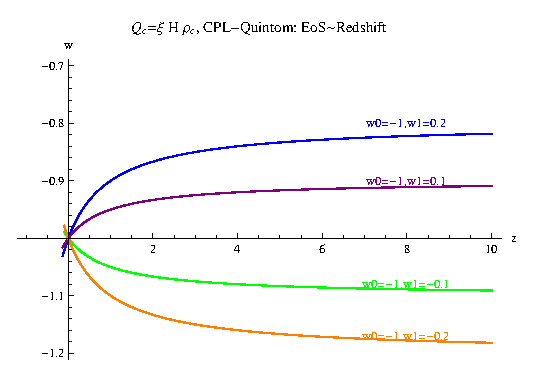
\includegraphics[width=250pt]{rhoc_ICCPL_Quintom_EoS1.eps}
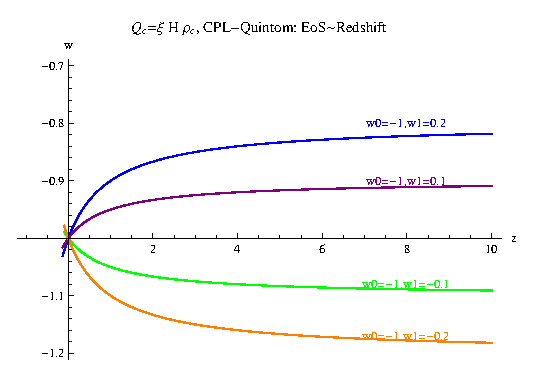
\includegraphics[width=250pt]{rhoc_ICCPL_Quintom_EoS1.eps}
\caption{The EoS}\label{fig-rhoc_ICCPL_Quintom_EoS}
\end{figure}




\begin{figure}
\centering
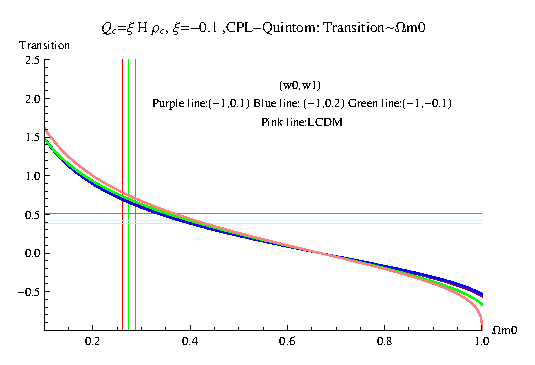
\includegraphics[width=250pt]{rhoc_ICCPL_Quintom_TransVSOmegam01.eps}
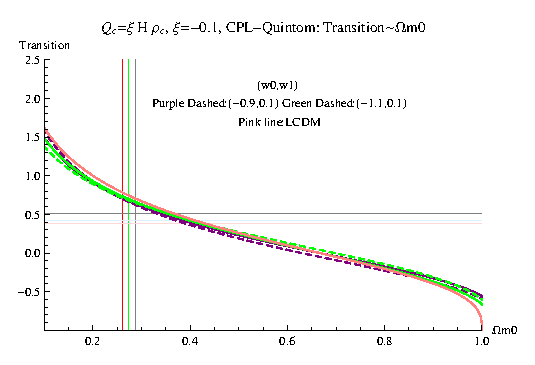
\includegraphics[width=250pt]{rhoc_ICCPL_Quintom_TransVSOmegam02.eps}
\caption{Transition vs $\Omega m0$}\label{fig-rhoc_ICCPL_Quintom_TransVSOmegam0}
\end{figure}

The left figure in \ref{fig-rhoc_ICCPL_Quintom_TransVSOmegam0} indicates a possible stationary point.\footnote{Only possible because I can only partially prove there is a nearly stationary. This is on my \CN .}


\begin{figure}
\centering
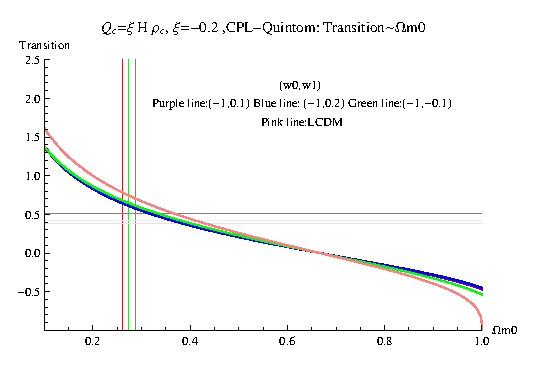
\includegraphics[width=250pt]{rhoc_ICCPL_Quintom_TransVSOmegam021.eps}
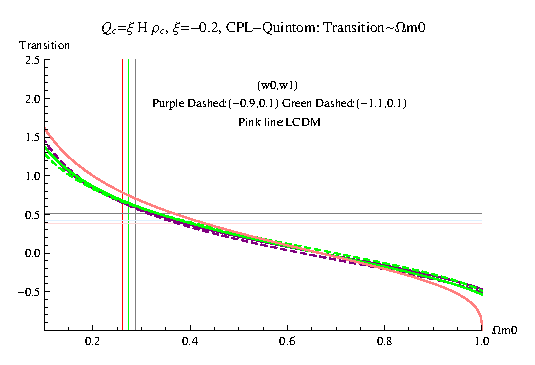
\includegraphics[width=250pt]{rhoc_ICCPL_Quintom_TransVSOmegam022.eps}
\caption{Transition vs $\Omega m0$}\label{fig-rhoc_ICCPL_Quintom_TransVSOmegam02}
\end{figure}



\begin{figure}
\centering
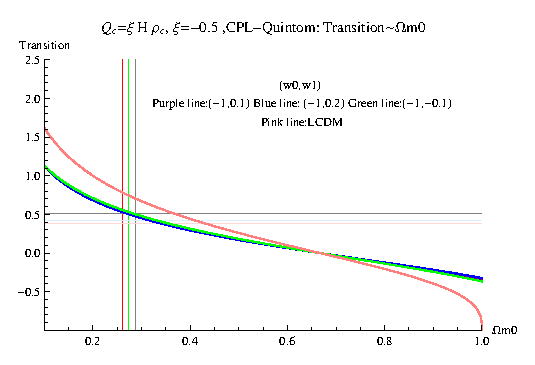
\includegraphics[width=250pt]{rhoc_ICCPL_Quintom_TransVSOmegam051.eps}
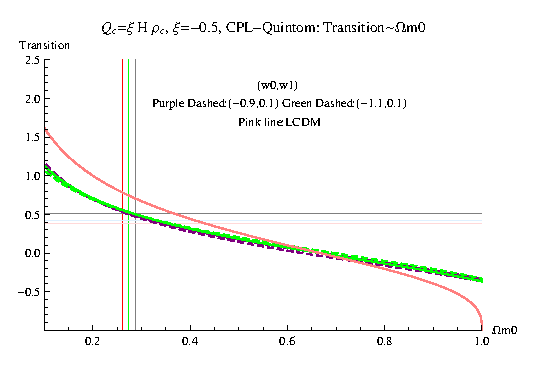
\includegraphics[width=250pt]{rhoc_ICCPL_Quintom_TransVSOmegam052.eps}
\caption{Transition vs $\Omega m0$}\label{fig-rhoc_ICCPL_Quintom_TransVSOmegam05}
\end{figure}


Comparing figure \ref{fig-rhoc_ICCPL_Quintom_TransVSOmegam05}, figure \ref{fig-rhoc_ICCPL_Quintom_TransVSOmegam02} and figure \ref{fig-rhoc_ICCPL_Quintom_TransVSOmegam0}, it seems that all lines cross point (0.66, 0), the reason of which, however, is because $w0=-1$ and a small nearly zero $w1$ means a similar evolution with $Q_c=\xi H\rho_c$ with a constant EoS. \footnote{The lines do not intercept with each other at the same point actually.}

\begin{figure}
\centering
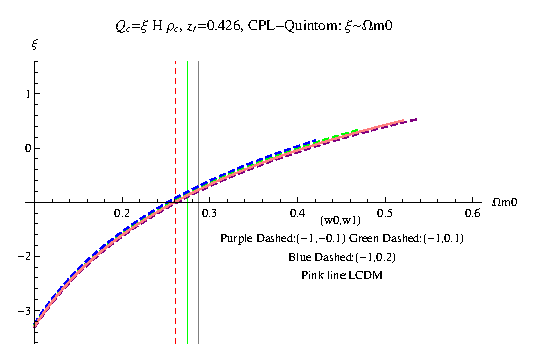
\includegraphics[width=250pt]{rhoc_ICCPL_Quintom_xiVSOmegam01.eps}
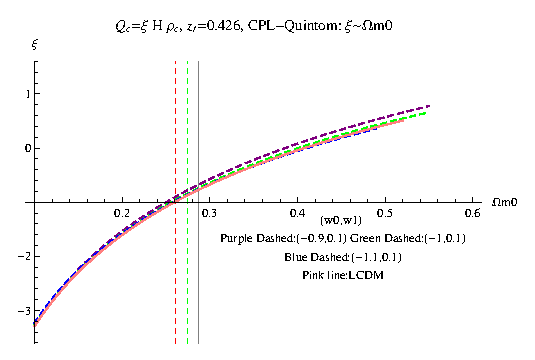
\includegraphics[width=250pt]{rhoc_ICCPL_Quintom_xiVSOmegam02.eps}
\caption{$\xi$ vs $\Omega m0$}\label{fig-rhoc_ICCPL_Quintom_xiVSOmegam0}
\end{figure}



(Other results are shown on the complete results files.)



0
\subsubsection{Quintessence}

(Figures \ref{fig-rhoc_ICCPL_Quint_EoS}, \ref{fig-rhoc_ICCPL_Quint_TransVSOmegam0} and \ref{fig-rhoc_ICCPL_Quint_xiVSOmegam0}. )

\begin{figure}
\centering
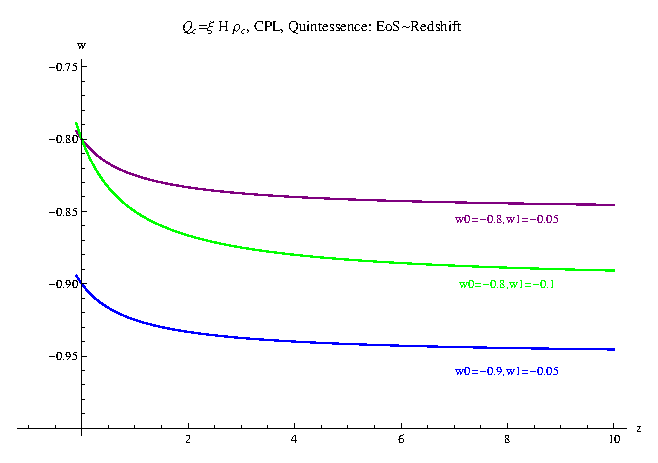
\includegraphics[width=500pt]{rhoc_ICCPL_Quint_EoS.eps}
\caption{The EoS}\label{fig-rhoc_ICCPL_Quint_EoS}
\end{figure}

\begin{figure}
\centering
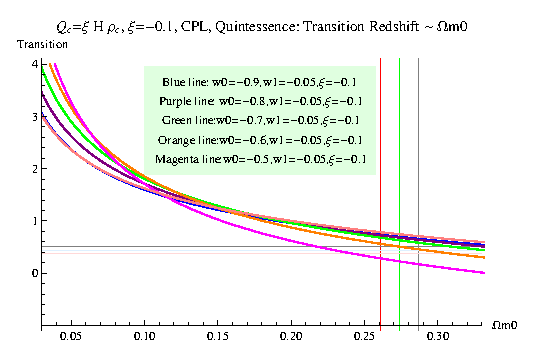
\includegraphics[width=250pt]{rhoc_ICCPL_Quint_TransVSOmegam01.eps}
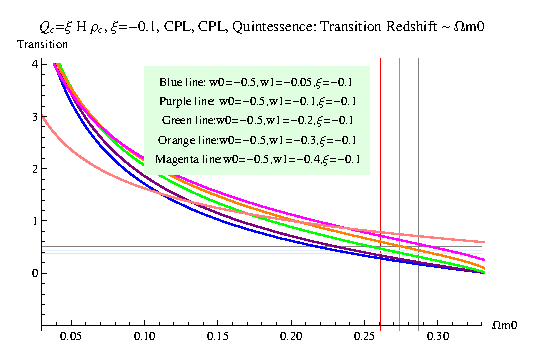
\includegraphics[width=250pt]{rhoc_ICCPL_Quint_TransVSOmegam02.eps}
\caption{Transition vs $\Omega m0$}\label{fig-rhoc_ICCPL_Quint_TransVSOmegam0}
\end{figure}

There is a features in the right figure of \ref{fig-rhoc_ICCPL_Quint_TransVSOmegam0}. The difference between lines become smaller when $\Omega m0$ is small and at about 0.35. Reason for this is when $\Omega m0$ is smaller, the evolution is mainly determined by $\Omega d$ (\footnote{In the solutions of $\rho_c$ and $\rho_d$, it is clear that $\Omega m0$ determines how much $w1$ will affect the result because the term $e^{3w1\frac{1}{1+z}}$ is small since $w1$ and $1/(1+z)$ are small and $\Omega m0$ is the amplitude of the other term in which $w1$ is in charge. Check \CN .})


\begin{figure}
\centering
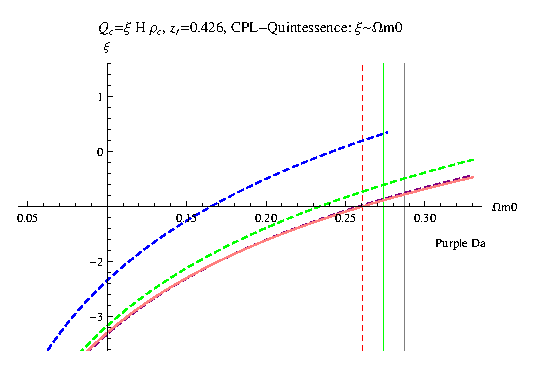
\includegraphics[width=250pt]{rhoc_ICCPL_Quint_xiVSOmegam01.eps}
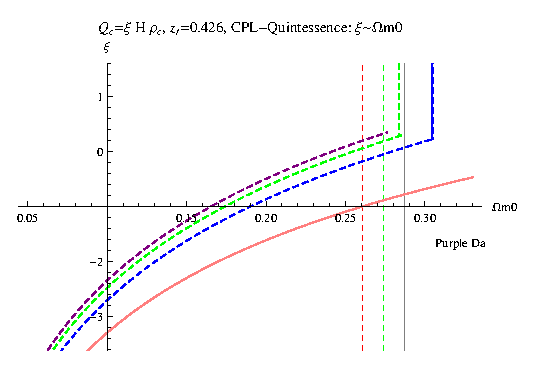
\includegraphics[width=250pt]{rhoc_ICCPL_Quint_xiVSOmegam02.eps}
\caption{$\xi$ vs $\Omega m0$}\label{fig-rhoc_ICCPL_Quint_xiVSOmegam0}
\end{figure}




\subsubsection{Phantom}

(Figures \ref{fig-rhoc_ICCPL_Phan_EoS}, \ref{fig-rhoc_ICCPL_Phan_TransVSOmegam0}, \ref{fig-rhoc_ICCPL_Phan_xiVSOmegam0})

\begin{figure}
\centering
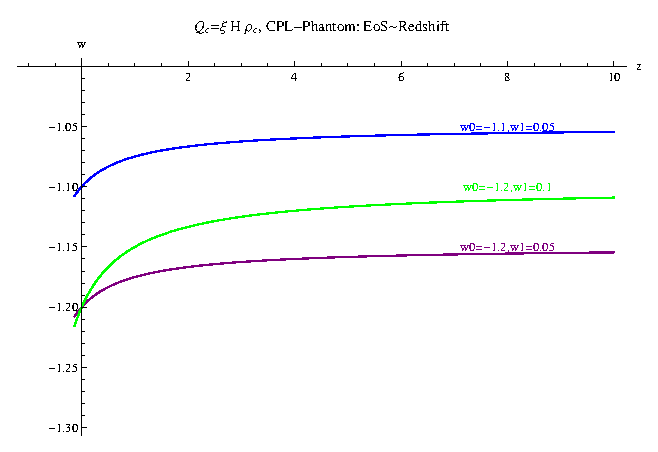
\includegraphics[width=500pt]{rhoc_ICCPL_Phan_EoS.eps}
\caption{The EoS}\label{fig-rhoc_ICCPL_Phan_EoS}
\end{figure}

\begin{figure}
\centering
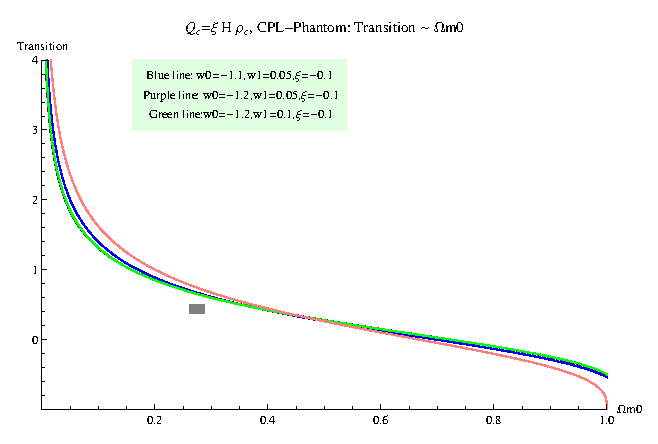
\includegraphics[width=500pt]{rhoc_ICCPL_Phan_TransVSOmegam0.eps}
\caption{Transition vs $\Omega m0$}\label{fig-rhoc_ICCPL_Phan_TransVSOmegam0}
\end{figure}



\begin{figure}
\centering
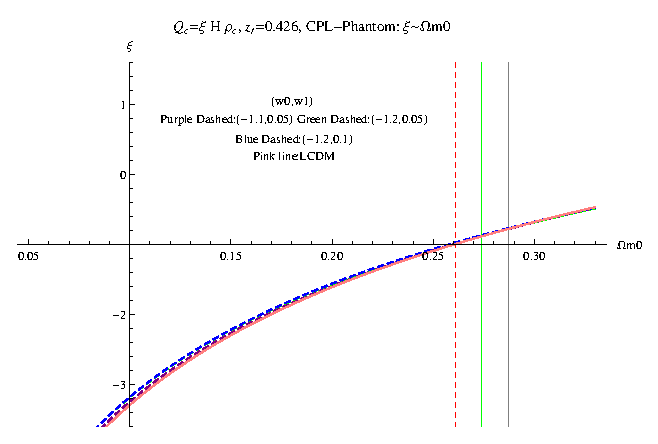
\includegraphics[width=500pt]{rhoc_ICCPL_Phan_xiVSOmegam0.eps}
\caption{$\xi$ vs $\Omega m0$}\label{fig-rhoc_ICCPL_Phan_xiVSOmegam0}
\end{figure}










\subsection{$Q_c=\xi H \rho_d$}


(Figures \ref{fig-rhod_I2CC_DecPara}, \ref{fig-rhod_I2CC_TransVSOmegam0}, \ref{fig-rhod_I2CC_xiVSw}, \ref{fig-rhod_I2CC_xiVSw2})

\begin{figure}
\centering
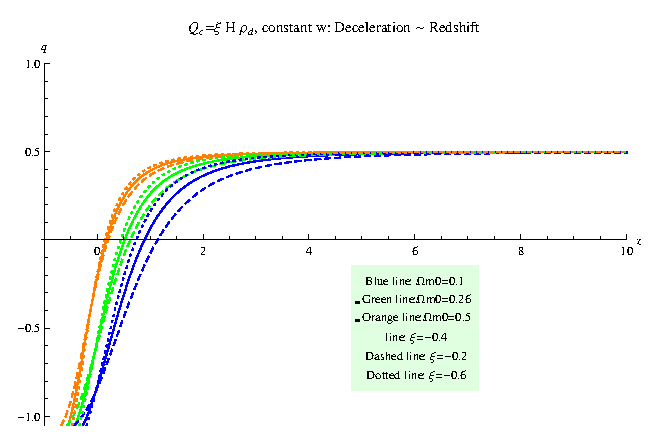
\includegraphics[width=500pt]{rhod_I2CC_DecPara.eps}
\caption{Deceleration parameter}\label{fig-rhod_I2CC_DecPara}
\end{figure}

\begin{figure}
\centering
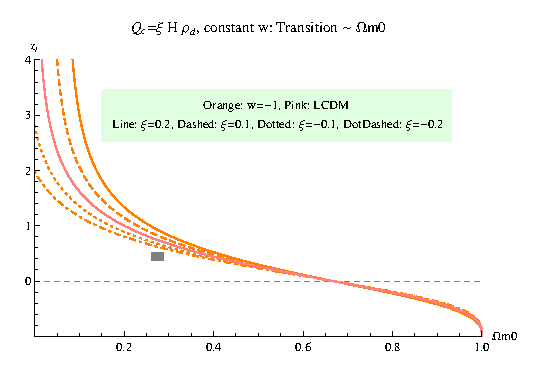
\includegraphics[width=250pt]{rhod_I2CC_TransVSOmegam01.eps}
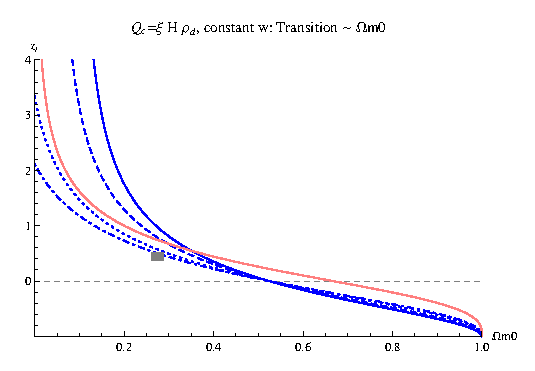
\includegraphics[width=250pt]{rhod_I2CC_TransVSOmegam02.eps}
\caption{Transition vs $\Omega m0$. For a flat universe, choose the parameters {w0=-1.02,w1=0.6}, the region for interation cosntant $\xi$ should be  (-1.04,-0.21) with a center at -0.64, derived from the (transition redshift, $\Omega m0$) plane, while a result of (-1.01, -0.23) with a center at -0.63, derived from (transition redshift, $\Omega m0$/$\Omega d0$) plane.}\label{fig-rhod_I2CC_TransVSOmegam0}
\end{figure}



\begin{figure}
\centering
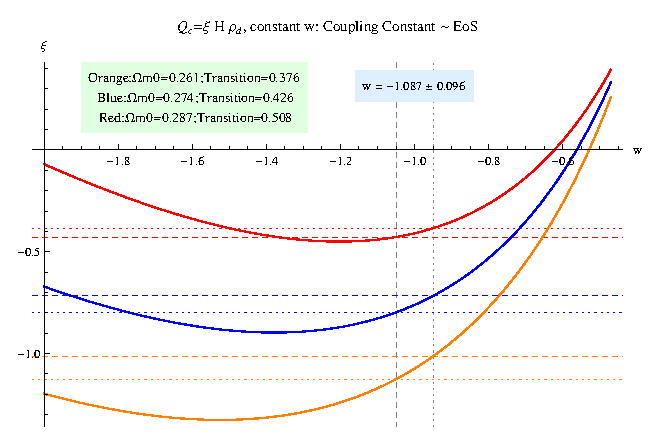
\includegraphics[width=500pt]{rhod_I2CC_xiVSw.eps}
\caption{$\xi$ VS $w$}\label{fig-rhod_I2CC_xiVSw}
\end{figure}

\begin{figure}
\centering
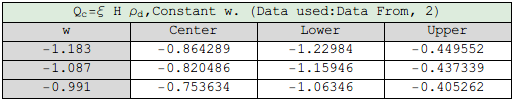
\includegraphics[width=450pt]{rhod_I2CC_table1.png}
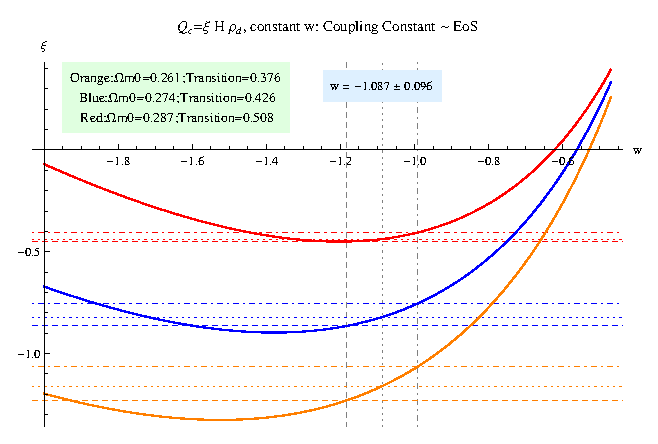
\includegraphics[width=500pt]{rhod_I2CC_xiVSw2.eps}
\caption{$\xi$ VS $w$}\label{fig-rhod_I2CC_xiVSw2}
\end{figure}




\begin{figure}
\centering
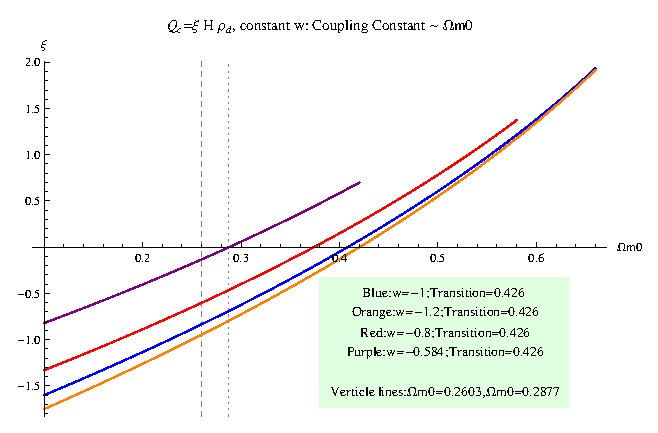
\includegraphics[width=500pt]{rhod_I2CC_xiVSOmegam02.eps}
\caption{$\xi$ VS $\Omega m0$}\label{fig-rhod_I2CC_xiVSOmegam02}
\end{figure}





\subsection{I2CCPL}

(Figures \ref{fig-rhod_I2CCPL_DecPara}, \ref{fig-rhod_I2CCPL_TransVSOmegam0})


\begin{figure}
\centering
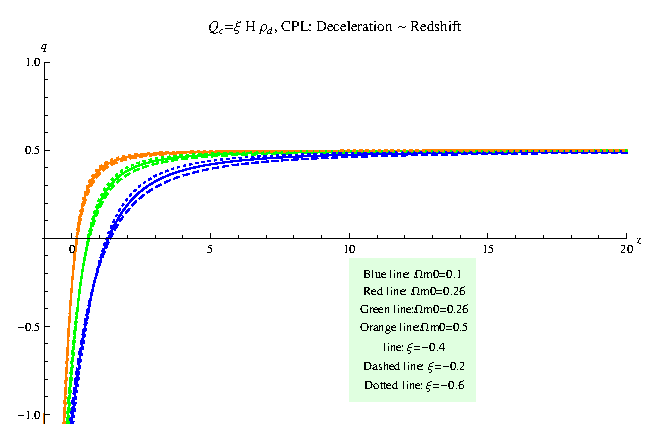
\includegraphics[width=500pt]{rhod_I2CCPL_DecPara.eps}
\caption{Deceleration parameter}\label{fig-rhod_I2CCPL_DecPara}
\end{figure}

Figure \ref{fig-rhod_I2CCPL_DecPara} shows the all the deceleration are the same at very early time. 




\begin{figure}
\centering
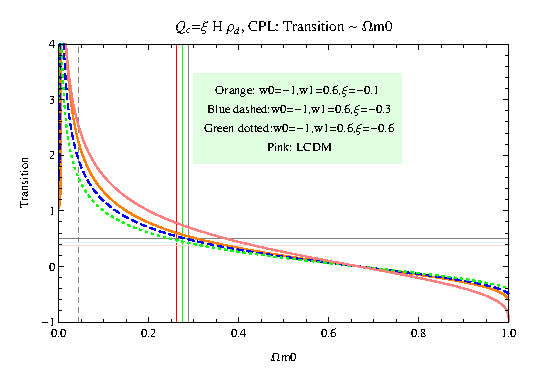
\includegraphics[width=250pt]{rhod_I2CCPL_TransVSOmegam01.eps}
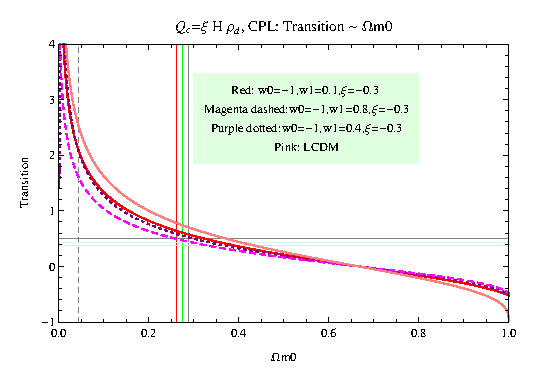
\includegraphics[width=250pt]{rhod_I2CCPL_TransVSOmegam02.eps}
\caption{Transition VS $\Omega m0$}\label{fig-rhod_I2CCPL_TransVSOmegam0}
\end{figure}


\subsubsection{Quintom}

(Figures \ref{fig-rhod_I2CCPL_Quintom_TransVSOmegam0}, \ref{fig-rhod_I2CCPL_Quintom_xiVSOmegam0})

\begin{figure}
\centering
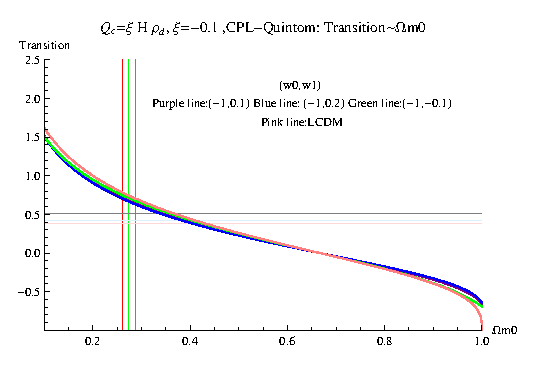
\includegraphics[width=250pt]{rhod_I2CCPL_Quintom_TransVSOmegam01.eps}
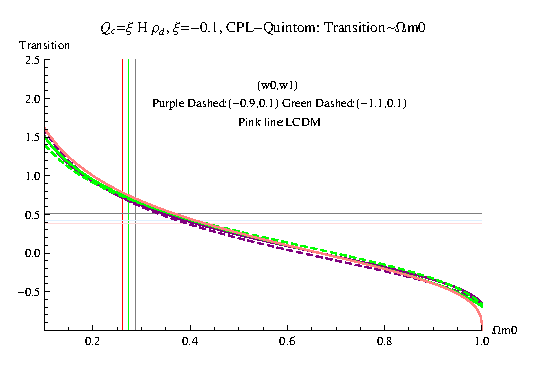
\includegraphics[width=250pt]{rhod_I2CCPL_Quintom_TransVSOmegam02.eps}
\caption{Transition VS $\Omega m0$}\label{fig-rhod_I2CCPL_Quintom_TransVSOmegam0}
\end{figure}



\begin{figure}
\centering
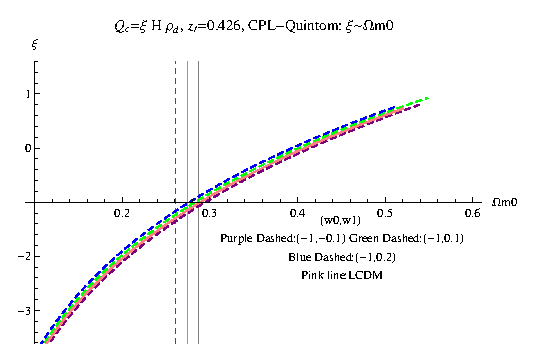
\includegraphics[width=250pt]{rhod_I2CCPL_Quintom_xiVSOmegam01.eps}
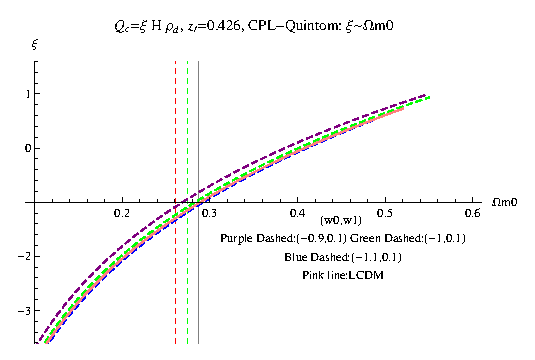
\includegraphics[width=250pt]{rhod_I2CCPL_Quintom_xiVSOmegam02.eps}
\caption{$\xi$ VS $\Omega m0$}\label{fig-rhod_I2CCPL_Quintom_xiVSOmegam0}
\end{figure}



\subsubsection{Quintessence}

(Figures \ref{fig-rhod_I2CCPL_Quint_TransVSOmegam0}, \ref{fig-rhod_I2CCPL_Quint_xiVSOmegam0})

\begin{figure}
\centering
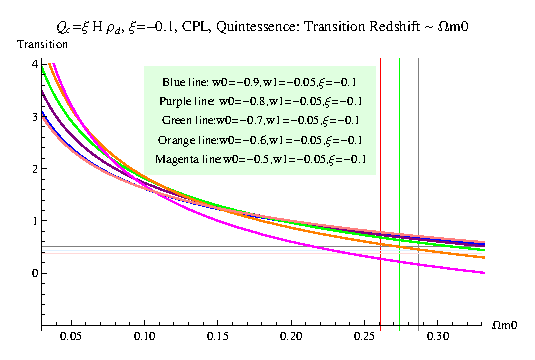
\includegraphics[width=250pt]{rhod_I2CCPL_Quint_TransVSOmegam01.eps}
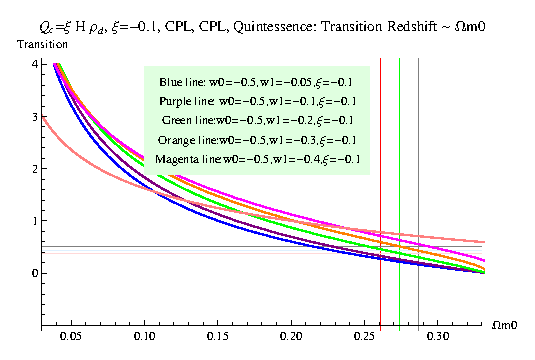
\includegraphics[width=250pt]{rhod_I2CCPL_Quint_TransVSOmegam02.eps}
\caption{Transition VS $\Omega m0$}\label{fig-rhod_I2CCPL_Quint_TransVSOmegam0}
\end{figure}



\begin{figure}
\centering
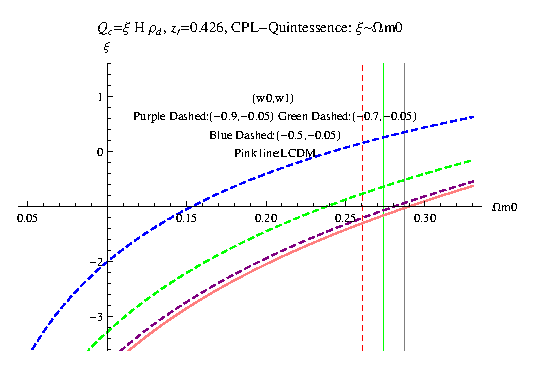
\includegraphics[width=250pt]{rhod_I2CCPL_Quint_xiVSOmegam01.eps}
\includegraphics[width=250pt]{rhod_I2CCPL_Quint_xiVSOmegam02.eps}
\caption{$\xi$ VS $\Omega m0$}\label{fig-rhod_I2CCPL_Quint_xiVSOmegam0}
\end{figure}






\subsubsection{Phantom}

(Figures \ref{fig-rhod_I2CCPL_Phan_TransVSOmegam0}, \ref{fig-rhod_I2CCPL_Phan_xiVSOmegam0})



\begin{figure}
\centering
\includegraphics[width=500pt]{rhod_I2CCPL_Phan_TransVSOmegam0.eps}
\caption{Transition VS $\Omega m0$}\label{fig-rhod_I2CCPL_Phan_TransVSOmegam0}
\end{figure}



\begin{figure}
\centering
\includegraphics[width=500pt]{rhod_I2CCPL_Phan_xiVSOmegam0.eps}
\caption{Transition VS $\Omega m0$}\label{fig-rhod_I2CCPL_Phan_xiVSOmegam0}
\end{figure}



{\bf There is always a almost-stationary point.}








%\includegraphics{files/DataFitting2_07-28.pdf}
%\includegraphics{files/supplement_08-10.pdf}



\end{document}